\subsection{Results}
In the subsequent analysis, we use the Weighted Interval Score (WIS) to quantify our forecasting performance. To reiterate, the WIS we used evaluates the distance between the projected distribution and the target value at the log scale. The arithmetic mean of WIS considers relative error on the log scale, which is equivalent to the geometric mean. $\exp(\text{WIS}) - 1$ offers an indication of the absolute relative error. The forecasting performance is compared to that of a baseline model, which is a flat-line projector that determines its median using 7-day moving average of the most recent observations. Therefore, the WIS of the baseline is simply the absolute error between the most recent observation and the finalized value at the log scale. 

We examine the performance of forecasting produced by our method for each of the three datasets described in Section 4.1. Since the MA-DPH confirmed case data are normalized by a constant (Massachusetts population), we only project the count of COVID-19 confirmed cases. For insurance claims data, we make forecasts of both the counts and the fractions of COVID-19 diagnosed outpatient insurance claims. For antigen test data, we make forecasts of the fractions of positive tests out of total tests. 

The following is a summary of the experimental results:
\begin{itemize}
    \item Our data revision forecasting framework substantially reduces forecast error, particularly when the lag is relatively small, e.g., the first 1-5 days. However, the gains in contribution tend to decrease as the lag increases. From this we conclude that modeling and correcting for data revisions may be most helpful when information is needed in close to real time.
    \item Comparing across the three datasets, we find that the task is most difficult for the insurance claims data, followed by antigent tests, and finally MA-DPH confirmed cases. Intuitively, this ordering matches Figure 1, where we observed that the claim data are the slowest of the three to converge.
    \item The abrupt distribution shift remains a problem. Our model relies on historical data revision patterns to forecast future updates, which entails the risk of introducing bias between the data revision pattern in the training dataset and the most recent data revision pattern. In cases where the data revision pattern undergoes a sudden and significant change within a short time period, particularly if such changes have not been previously observed, our model struggles in effectively adapting to these circumstances.
\end{itemize}

Next, we demonstrate the predictive performance of our model and how the performance varies along difference dimensions. 

\begin{figure}[h!]
    \centering
    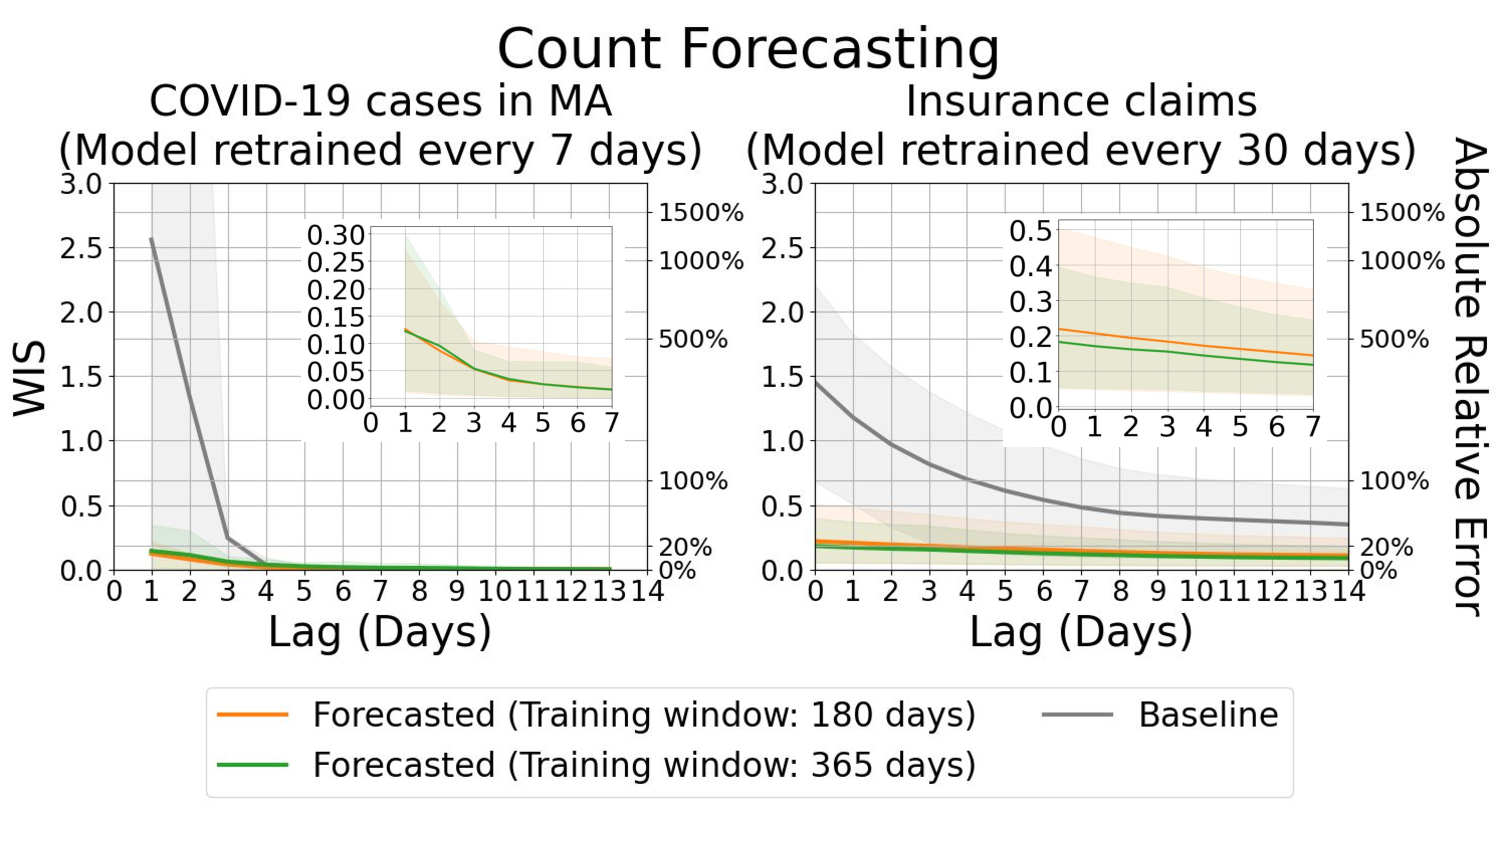
\includegraphics[width=\textwidth]{figs/experiment_count_result_evl_general.pdf}
    \caption{\emph{\textbf{Count rorecast evaluation results over lags.} Left: Forecasts of the number of finalized confirmed cases in Massachusetts only. Right: Forecasts of the number of insurance claims in all states based on insurance claims data. The solid lines represent the mean WIS, indicating the absolute relative errors between the most recent report and the target, averaged over locations and reference dates for each lag. The shaded areas represent the 10\% quantile to 90\% quantile.}}
\end{figure}

\begin{figure}[h!]
    \centering
    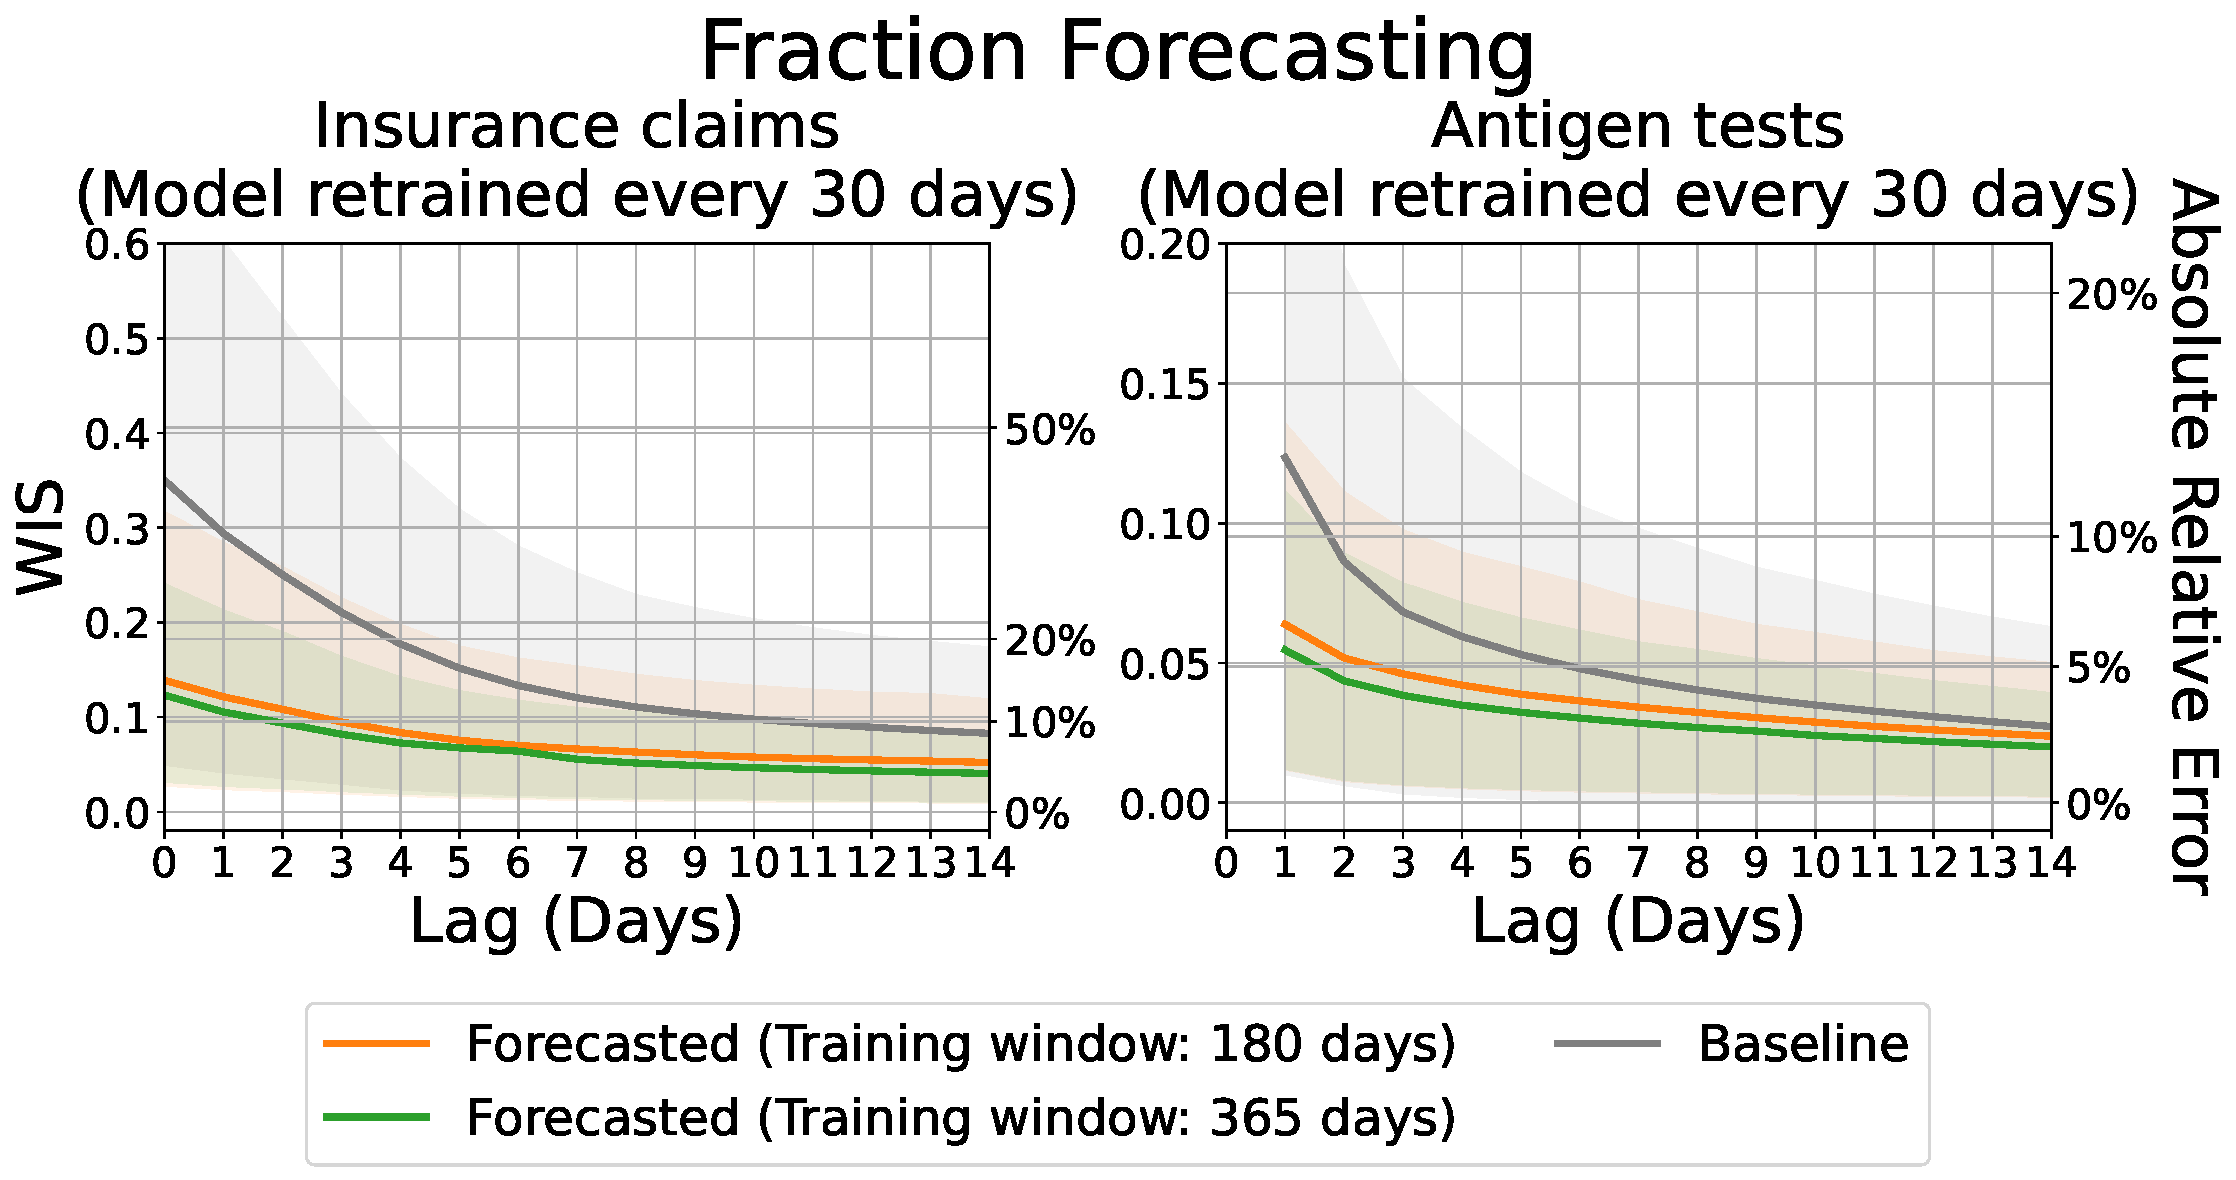
\includegraphics[width=\textwidth]{figs/experiment_frc_result_evl_general.pdf}
    \caption{\emph{\textbf{Fraction forecast evaluation results over lags.} Left: Forecasts of the fraction of COVID-19 insurance claims based on insurance claims data. Right: Forecasts of the fraction of positive COVID-19 antigen tests based on antigen tests data. The solid lines represent the mean WIS, indicating the absolute relative errors between the most recent report and the target, averaged over locations and reference dates for each lag. The shaded areas represent the 10\% quantile to 90\% quantile.}}
\end{figure}

\subsection{Aggregate Accuracy by Lag}
Here, study how the performance of the forecast varies as a function of the lag it is made at. When situated on date $s$ and using all the data available before $s$ to project $Y_{itL}$ based on $Y_{it(s-t)}$, we categorize it as a task with a lag of $s-t$.  Given that the data revision sequence of $Y_{it}$ gradually asymptotes to the finalized value, it follows that the smaller the lag, the more challenging the task. 

Figure 3 and Figure 4 present the evaluation results for the count and fraction forecasts, respectively, stratified by lag and averaged over all locations and reference dates. For confirmed case data (as shown in Figure 3, left panel), the mean absolute relative error of the baseline model initially starts at around 1400\% under this evaluation metric. However, the mean absolute relative error of the distribution forecasts is 20.40\% if using a 365-day training window or 15.68\% if using a 180-day training window. Our forecast results outperform the baseline, especially when the lag is smaller than 4. The performance gap is larger for insurance claim data, where revisions occur with greater frequency and variability. As shown in the right panel of Figure 3, the mean absolute relative error of the baseline remains larger than 30\% even after 14 days of revision. For our distributional forecast, the mean absolute relative error is only 24.52\% after just the first data release if using a 180-day training window and only 20.54\% if using a 365-day training window, with the performance improving further over time. 

Similarly, Figure 4 illustrates the mean absolute relative error of all COVID-19 fraction forecasts as a function of lag. For insurance claims data, the mean absolute relative error exceeds 30\% when comparing the first release (lag = 0) to the target (lag = 60). However, this error is reduced to 14.89\% using distributional forecasts with a 180-day training window and 13.10\% with a 365-day training window. Even after 7 days of revisions, the distributional forecast continues to yield substantial improvements. In contrast, antigen test data are much less affected by the data revision problem. However, even when provisional antigen test reports closely approximate the target, our framework still significantly reduces the mean absolute relative error, lowering it from 13.14\% to 6.59\% if using a 180-day training window and even to 5.62\% on average using a 365-day training window at the first release (lag=1).


\subsection{Aggregate Accuracy by Reference Date}

\begin{figure}[h!]
    \centering
    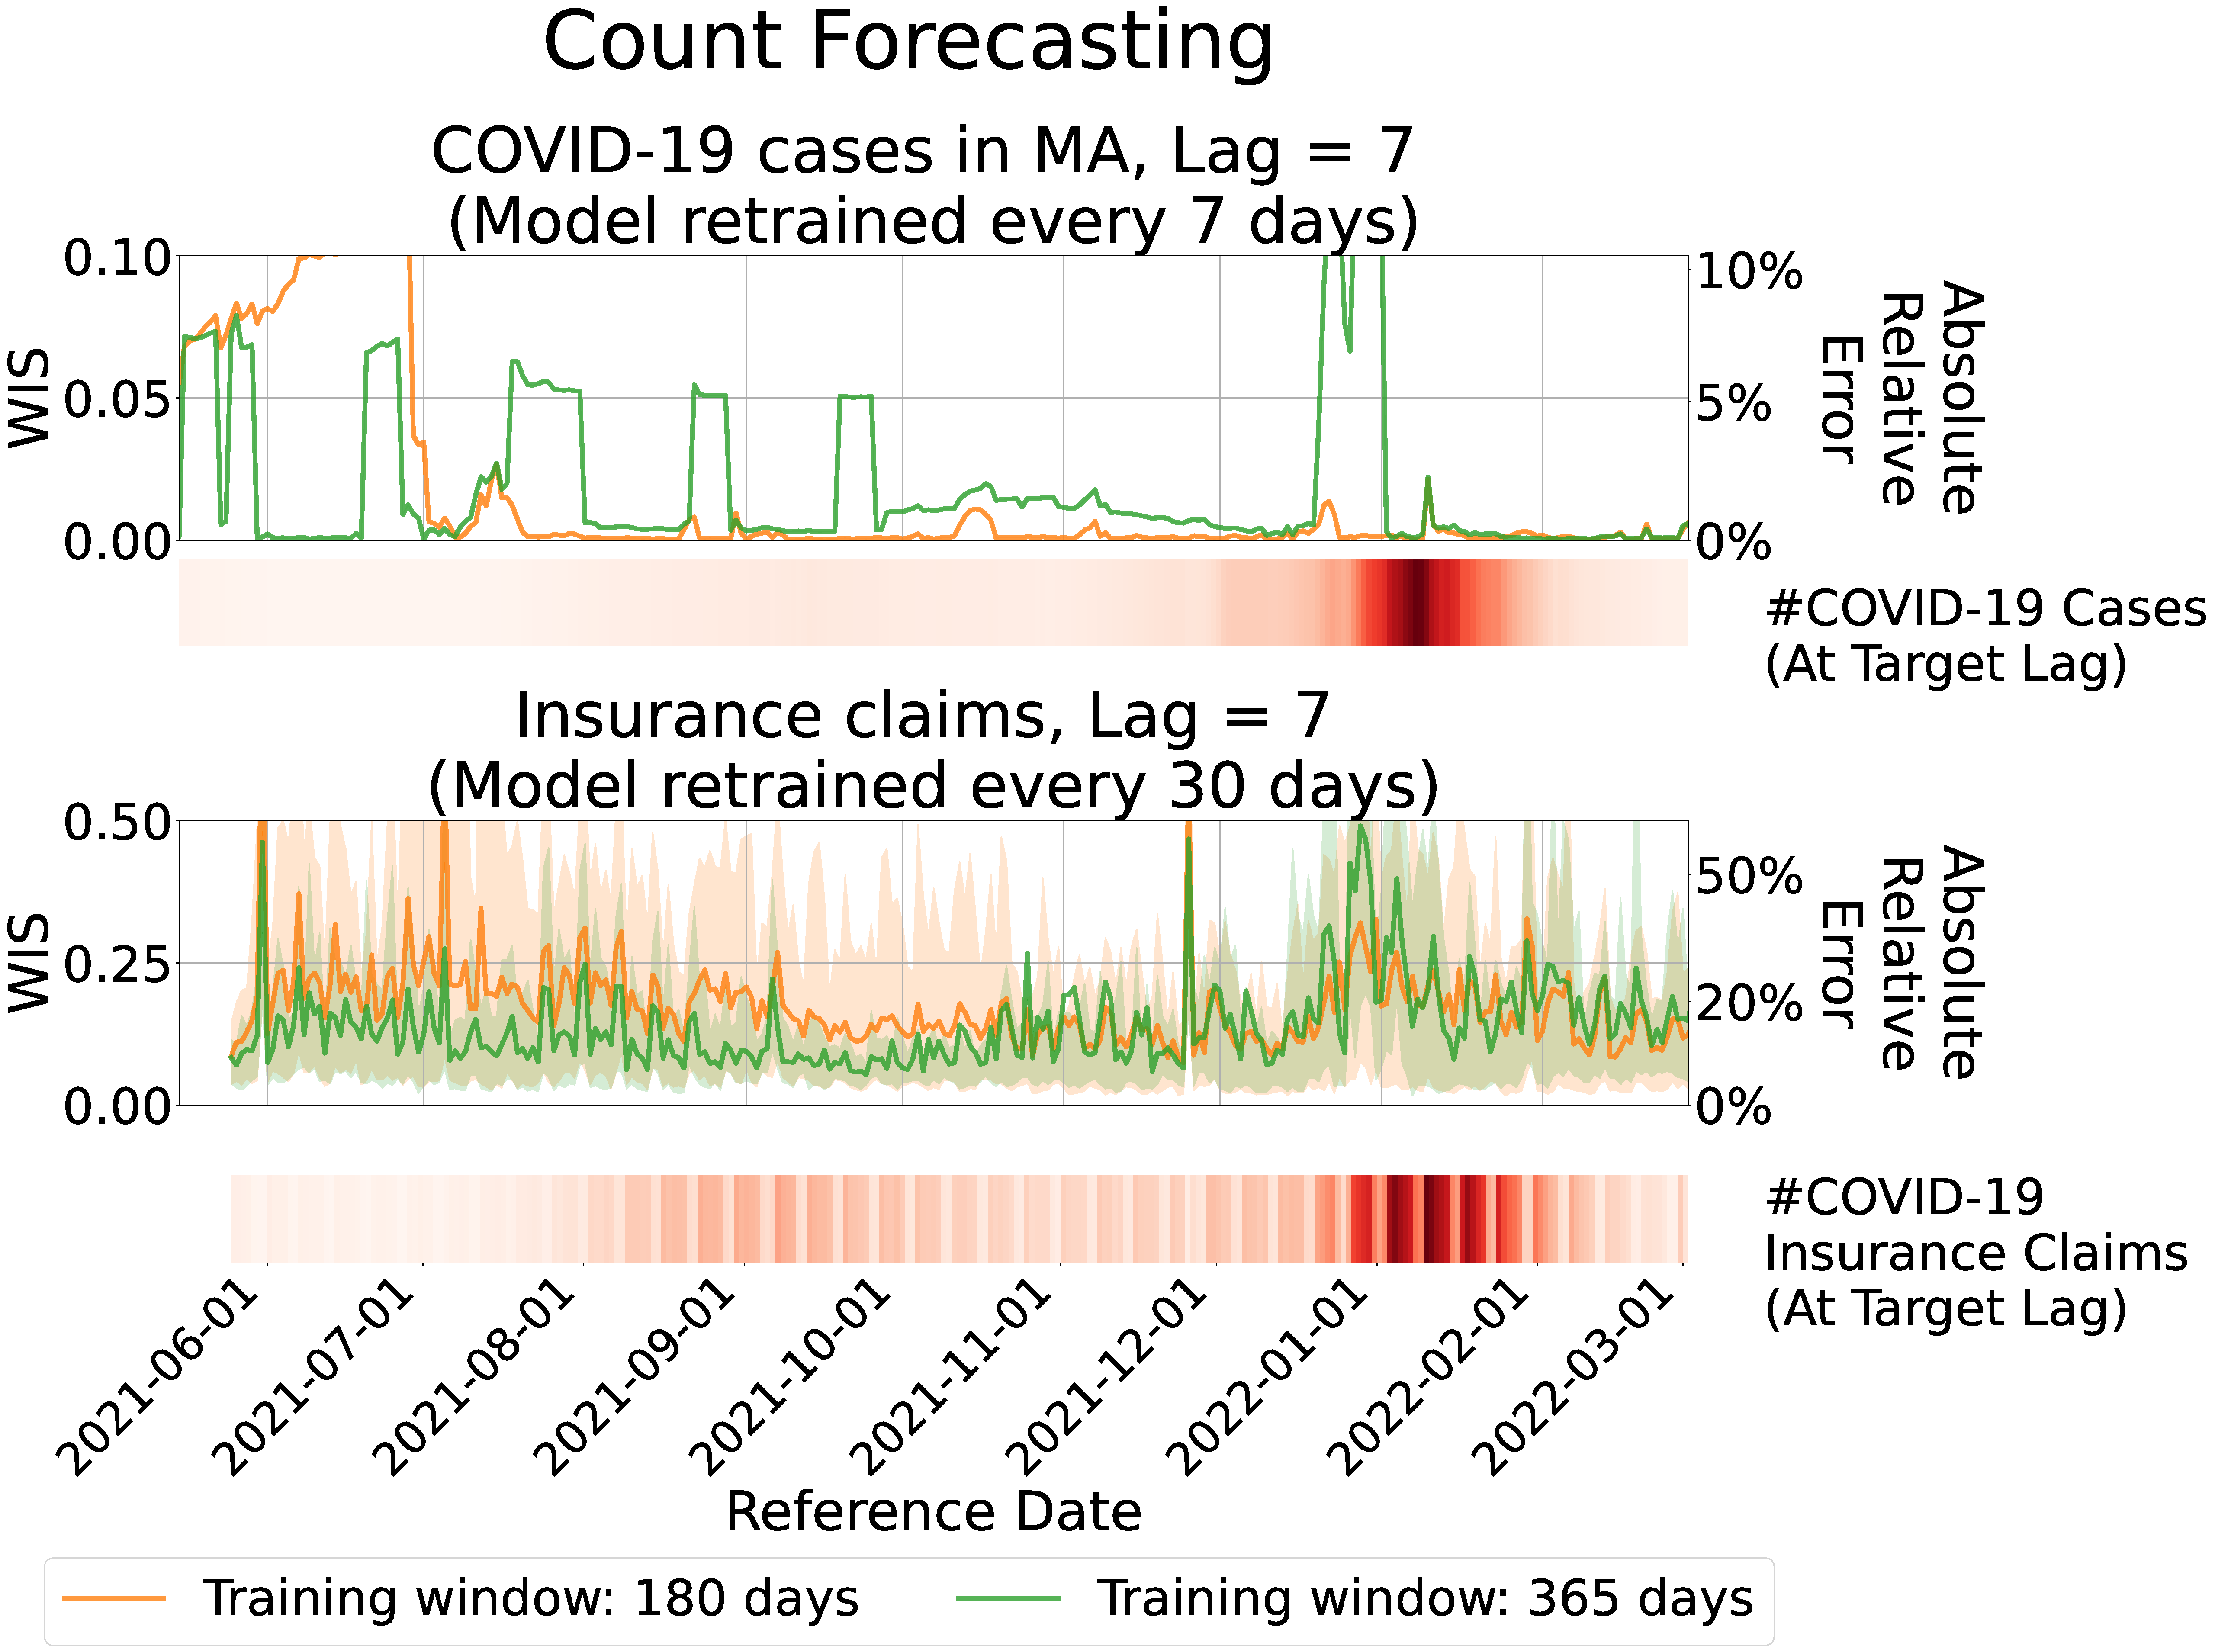
\includegraphics[width=\textwidth]{figs/experiment_count_result_time_series.pdf}
    \caption{\emph{\textbf{Count forecast evaluation results over reference dates.} Top: Forecasts of the number of finalized COVID-19 confirmed cases in Massachusetts only. Bottom: Forecasts of the number of COVID-19 insurance claims in all states based on insurance claims data. The solid lines represent the mean WIS at lag 7 averaged over locations for each reference date. The shaded areas represent the 10\% quantile to 90\% quantile. The heatmap illustrate the target values. Darker values indicate more cases/insurance claims.}}
\end{figure}

\begin{figure}[h!]
    \centering
    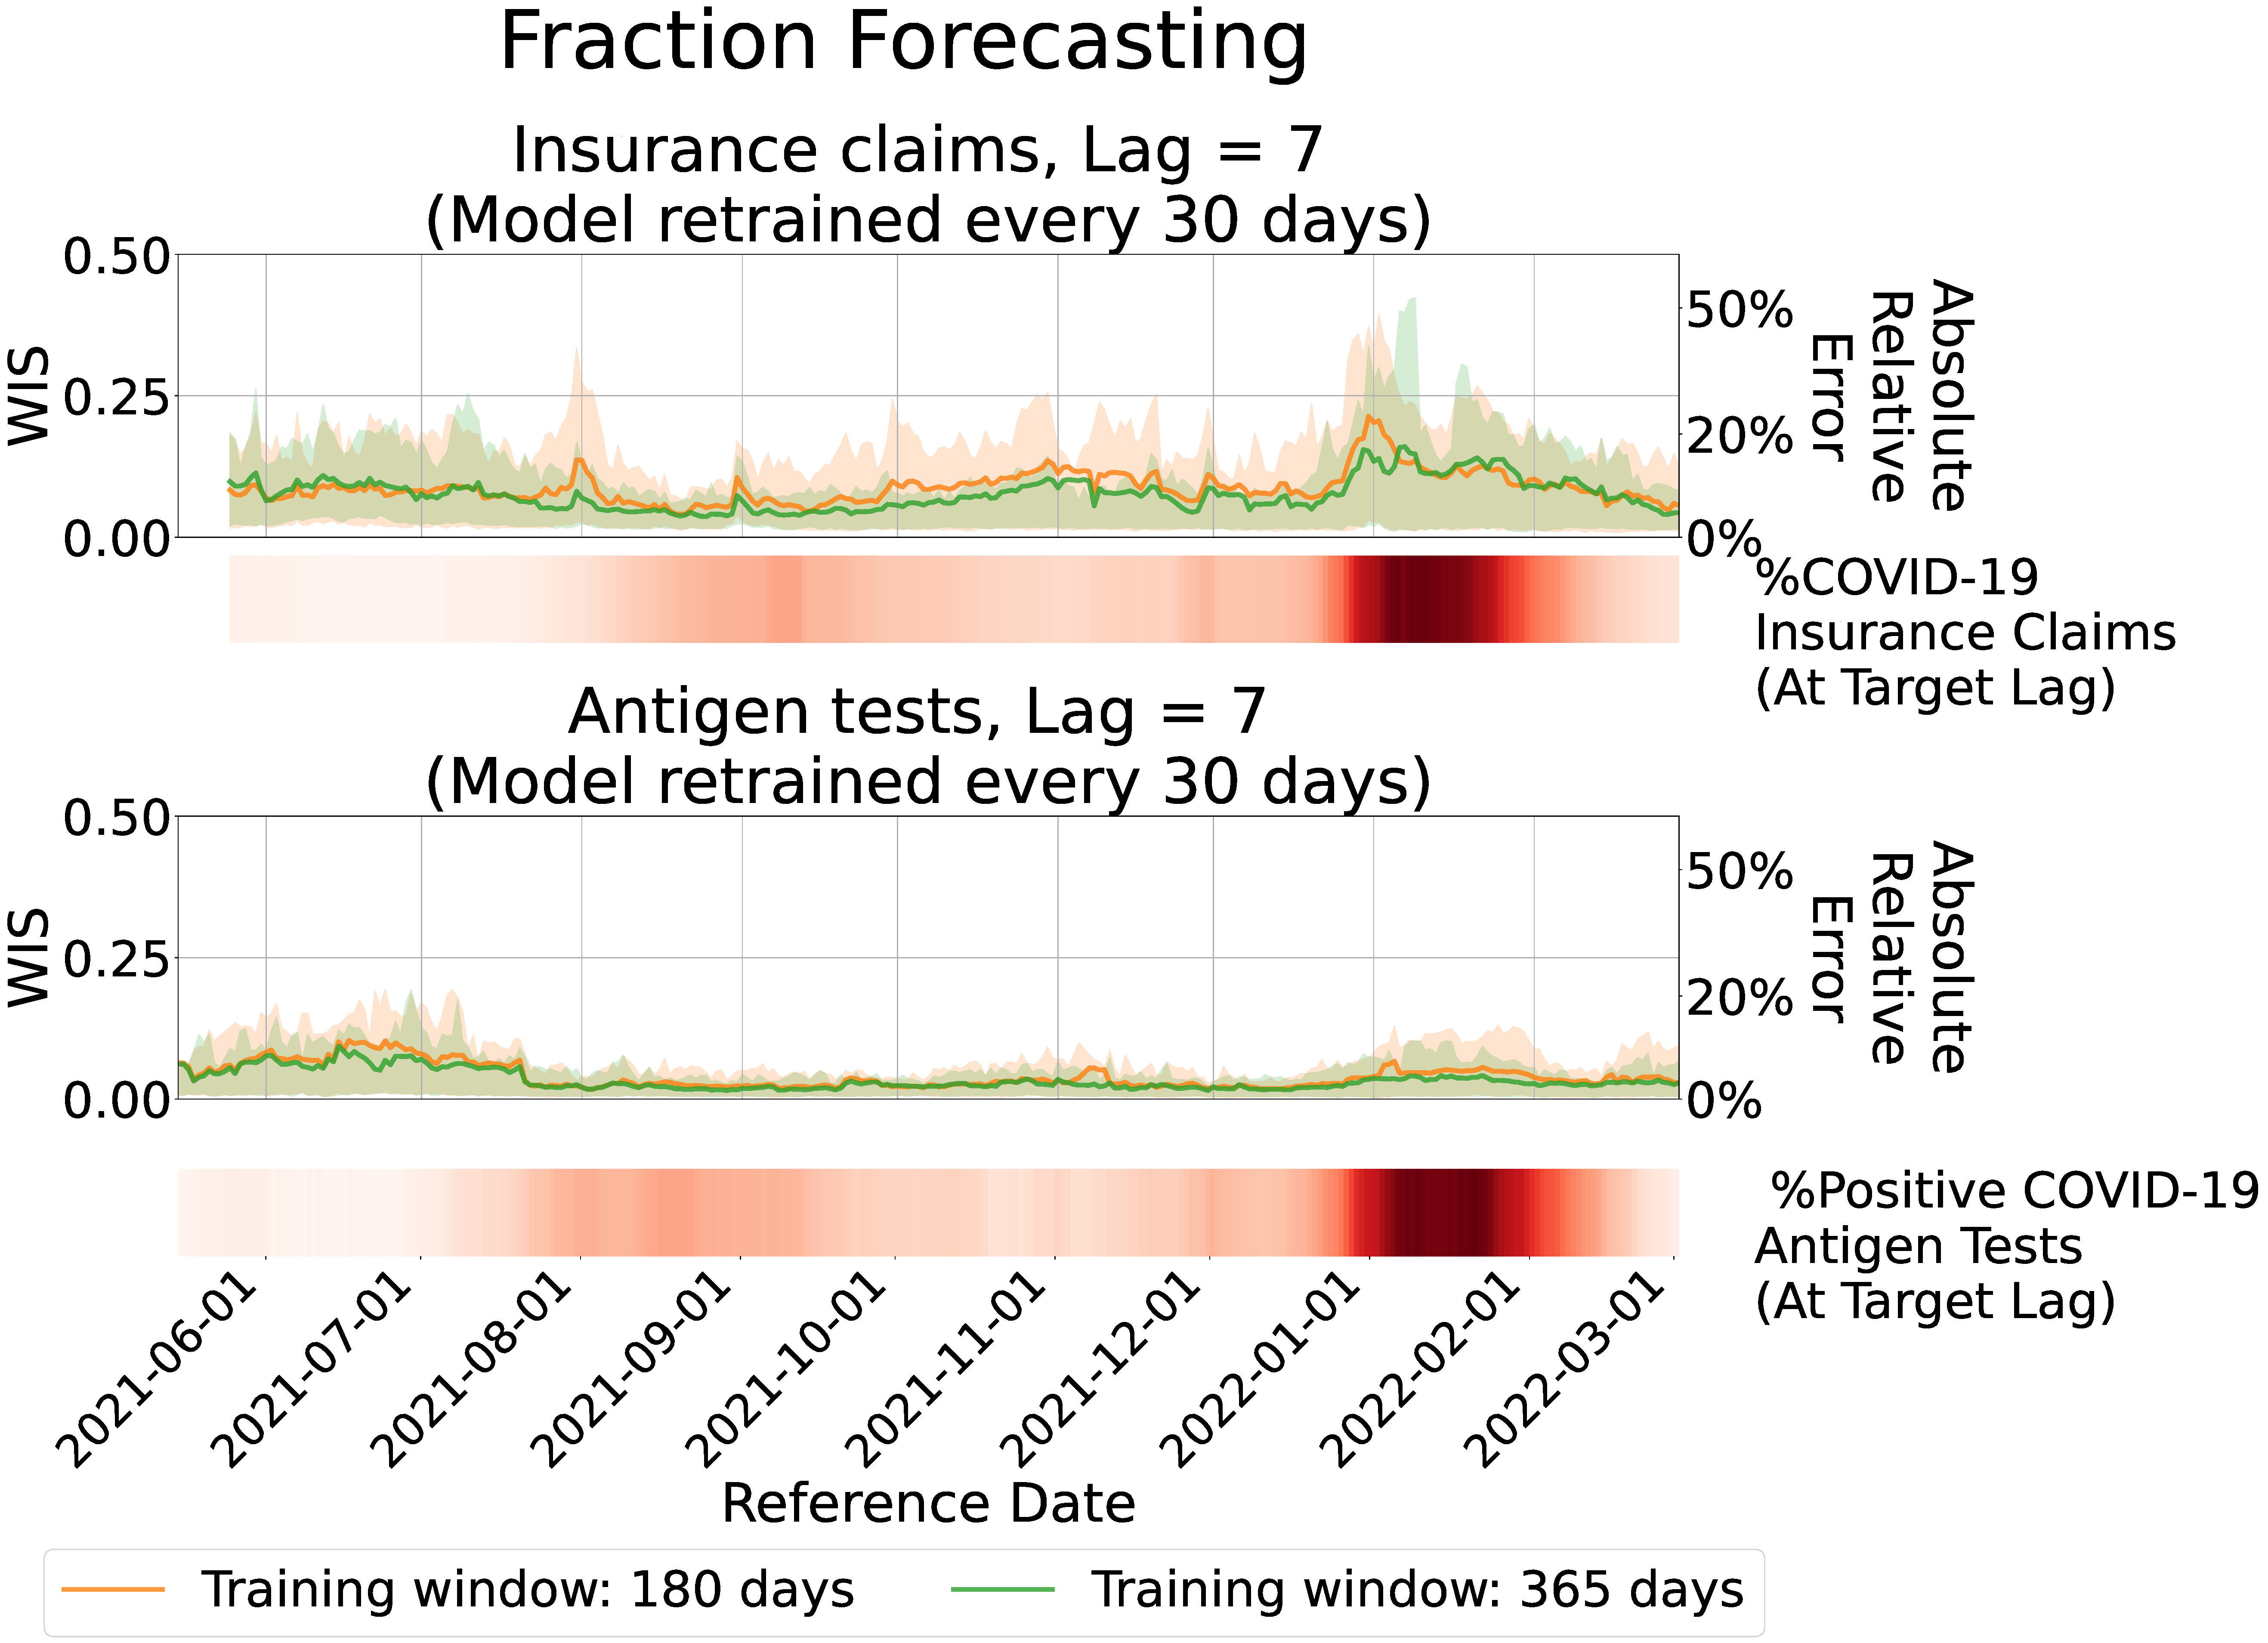
\includegraphics[width=\textwidth]{figs/experiment_fraction_result_time_series.pdf}
    \caption{\emph{\textbf{Fraction forecast evaluation results over reference dates.} Top: Forecasts of the fraction of COVID-19 insurance claims based on insurance claims data. Bottom: Forecasts of the fraction of positive COVID-19 antigen tests based on antigen tests data.  The solid lines represent the mean WIS at lag 7 averaged over locations for each reference date. The shaded areas represent the 10\% quantile to 90\% quantile. The heatmap illustrate the target values.}}
\end{figure}

The difficulty of the forecasting task varies not only across lag but also over time. Figure 5 and Figure 6 illustrate the evaluation results at lag 7 for count and fraction forecasts, respectively, stratified by reference date and averaged over all locations. The gray curves represent the national target surveillance values over time, with the exception of COVID-19 confirmed cases data, which pertain to Massachusetts only.

The target surveillance values exhibit two distinct waves: the Delta wave, occurring roughly from July to November 2021, and the Omicron wave, which spans from November 2021 to February 2022. During both waves, although generally well performing, our model's performance occasionally declines during periods of upswings and downswings. This is attributed to the lagging nature of our model, where coefficients derived from the data available L (the target lag) days ago introduce significant bias in the forecasts.

The Omicron wave represents the largest wave encountered during the COVID-19 pandemic, with infection rates reaching unprecedented levels and placing an enormous burden on the public health surveillance system. This surge also triggers abrupt and significant changes in the data revision pattern, posing a considerable challenge to our forecasting efforts, as the model struggles to forecast revision patterns never observed before.


Another challenging period is from June to July 2021, characterized by an extremely low general infection rate. Recall that the WIS consists of absolute deviations between the projected values and the target. This evaluation metric will exaggerate relative errors when the target is extremely small.


\subsection{Impact Factors of Forecast Accuracy}
Our model generally suffers in the two scenarios: 1) the period when there is an abrupt change in the target surveillance; 2) the period when the target values are extremely small. The first corresponds to the trend direction of the target surveillance curve, while the second corresponds to the level of target values. We now examine the distribution of WIS over lags, conditioned on the two factors, respectively.

The left penal of Figure 7 displays the distribution of WIS over the lags, where we stratify the data by whether there is a period of increasing fractions of COVID-19 insurance claims (up), decreasing fractions of COVID-19 insurance claims (down) or flat fractions of COVID-19 insurance claims(flat). The trend indicator is defined as follows: 
$$
    Z_{it}=
\begin{cases}
    1,           & \text{if } \frac{\widetilde{Y}_{itL}}{\widetilde{Y}_{i(t-7)(L+7)}} \geq 1.25\\
    0, & \text{if otherwise} \\    
    -1, & \text{if} \frac{\widetilde{Y}_{itL}}{\widetilde{Y}_{i(t-7)(L+7)}} \leq 0.75
\end{cases}
$$

$Z_{itl} = 1$ if the target surveillance value in the past 7 days has increased by at least 25\% compared to the previous week. When this occurs, we say that location $i$ at date $t$ has an upward trend. $Z_{itl} = -1$ if the target surveillance value in the past 7 days has decreased by at least 25\% compared to the previous week, indicating a downward trend.


\begin{figure}[h!]
    \centering
    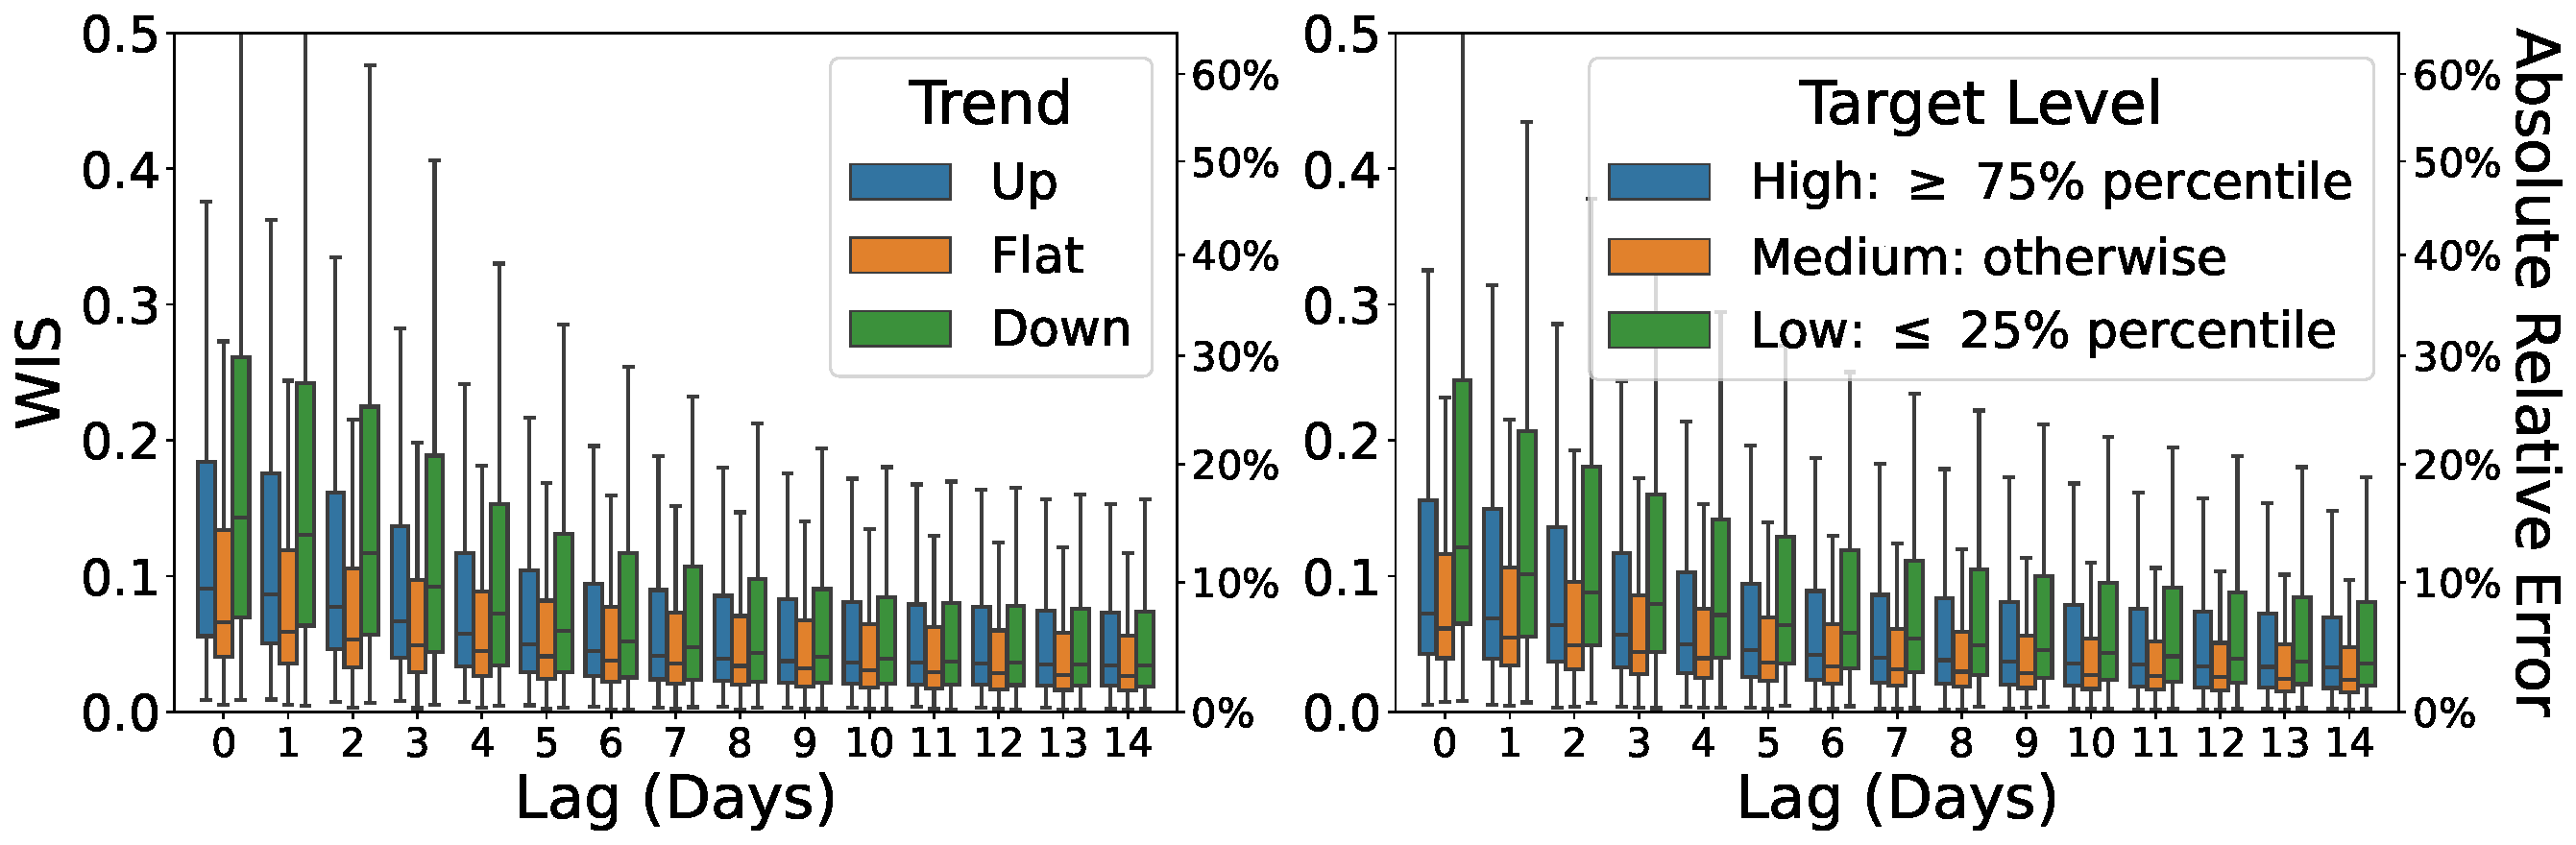
\includegraphics[width=\textwidth]{figs/experiment_fraction_result_factors.pdf}
    \caption{\emph{\textbf{Boxenplot illustrating the impact of various factors on the WIS} (each box conveys the level 25\%, 50\%, and 75\% quantiles of the WIS.) Left: forecasts stratified by whether the target surveillance trend is "Up", "Flat", or "Down". Right: forecasts stratified by whether the target surveillance value falls into the categories of "High", "Medium", or "Low".}}
\end{figure}

The forecasting performance notably improves during periods with no significant changes in the target surveillance curve. Surprisingly, the forecasting performance is poorest during down periods in the first week's revision. This is attributed to the fact that the "down" period comprises reference dates during the downswing of Omicron only, while the "up" period includes reference dates during the upswing of both Delta and Omicron. In general, the model performs relatively well during the Delta wave compared to the Omicron wave, since the distribution shift in the Delta wave is not as large as that in the Omicron wave. After the first 7 revisions, the performance gap across the three categories diminishes significantly, with the performance order changing to "Flat", "Down", "Up".

The right panel of Figure 7 illustrates the distribution of WIS over lags, stratified by whether the target surveillance value falls into the categories of "High", "Medium", or "Low". A target value is classified as "High" if it is greater than or equal to the 75\% percentile, while it is classified as "Low" if it is less than or equal to the 25\% percentile. The performance order, from best to worst, consistently ranks as "Medium", "High", "Low" across lags. Notably, even after the first 14 revisions, the performance gap across these three categories remains significant.


\subsection{Comparison of Performance with Alternative Methods}
In this section, we demonstrate that our model achieves comparable or superior forecast accuracy to nobBS \cite{McGough2020} and Epinowcast \cite{epinowcast}, while significantly reducing computational runtime. These two approaches were selected for comparison as they are among the most well-established methods, supported by existing R packages, and frequently cited in public health surveillance research.

Since both methods are specifically designed for count-type data, our comparison is limited to count-type datasets. For the insurance claim dataset with daily observations, we use a 180-day training window and a target lag of 60 days. To ensure a fair comparison, we apply the same 180-day moving window and a maximum delay of 60 days to nobBS and Epinowcast. To manage computational demands while maintaining consistency across models, we train all methods—including Delphi-RF—at 30-day intervals. Additionally, we evaluate performance on daily confirmed case data from MA-DPH, where revisions stabilize more quickly. For this dataset, we adjust the training frequency to every 7 days, set the maximum delay to 14 days, and maintain the 180-day moving window. In Delphi-RF, the target lag is also set to 14 days to align with these adjustments.

We further extended our comparison to weekly data. To ensure compatibility with weekly data, covariates containing daily change information were excluded. The full model is expressed as:

\begin{align*} 
Q_{f(Y_{itL}))|X_{itl}}^{\tau} &=  X_{itl}\beta^{\tau}\\
& = \beta_0^{\tau}  + \beta_{1}^{\tau}\mathbf{I}_{\text{first-week}(t+l)} &(\text{Intercept, week-of-month effects})\\ 
& + \beta_{2}^{\tau}f(Y_{itl}) + \beta_{3:5}^{\tau}\mathbf{e}_{\sqrt{Y_{itl}}} &(\text{Disease activity level}) \\ 
& + \beta_{6}^{\tau}f(Y_{i(t-7)(l+7)})+ \beta_{7}^{\tau}f(Y_{i(t-14)(l+14)}) \\
& + \beta_{8}^{\tau}f(Y_{i(t-7)l_{\text{min}}})+ \beta_{9}^{\tau}f(Y_{i(t-14)l_{\text{min}}})  &(\text{for the most recent changes}) \\ 
\end{align*}

where \(Y_{itl}\) represents the counts reported for the week spanning reference dates \(t-6\) to \(t\), as of the report date \(t+l\), for location \(i\). 

To further evaluate model performance across diverse surveillance settings, we tested the models in two additional datasets with distinct characteristics to assess their robustness. First, we used Puerto Rico (PR) dengue weekly surveillance data from 1991-12-23 to 2010-11-29 (989 weeks). This dataset, characterized by a long historical record and strong seasonality, differs from the more irregular trends observed in COVID-19 data. By applying our method to dengue data, we can assess its ability to adapt to seasonal fluctuations and long-term surveillance trends. The target lag was set to 10 weeks, and 104 weeks of data were used for training. For comparison, we generated weekly forecasts using the nobBS and Epinowcast models over the same time periods. In these experiments, the maximum delay was set to 10 weeks and a 104-week moving window was applied, consistent with the setup in \cite{McGough2020}. For all three models, training and forecasting were performed on a weekly basis. 

We also tested the models on national weekly ILI data from 2014-06-30 to 2017-09-25 (170 weeks), which follows a different reporting pattern. For Delphi-RF, a 27-week training dataset was used, with a target lag of 26 weeks. The maximum delay was set to 26 weeks and a 27-week moving window was used for nobBS and Epinowcast. 

The experiments were conducted on an Apple Mac Pro with a 3 GHz 6-Core Intel Core i5 processor, running macOS Sequoia Version 15.2, and using R version 4.4.2.

\begin{table}[h!]
\centering
\resizebox{\textwidth}{!}{%

\begin{tabular}{cc|cccc}
\hline
\multicolumn{2}{c|}{\multirow{2}{*}{\makecell{\textbf{Computing Time(s)}\\(per location per report date)}}} & \multicolumn{4}{c}{\textbf{Model}}  \\
                     & &Delphi-RF Training\\ & &(only once per\\ & & week or month) & Delphi-RF Testing &Epinowcast &nobBS\\
\hline
\multirow{6}{*}{\rotatebox{90}{\textbf{Dataset}}} &\makecell{Confirmed Cases\\(Daily, State, MA only)} & $5.921 \pm 0.539$ &$0.369\pm 0.006$  &$181.583\pm 16.778$ &$22.611\pm 1.093$ \\
&\makecell{Insurance Claims \\ (Daily, State)}   & $43.936\pm 0.025$ &$0.819\pm 0.008$&$579.540 \pm 14.096$ &$96.030 \pm  0.431$ \\
 
% &\makecell{Insurance Claims\\(Weekly, State)} &$0.408 \pm 0.001$ &$0.003\pm 0.000$ &$10.332 \pm 0.129$ &$1.638 \pm 0.002$ \\ 
 &\makecell{Dengue Fever Cases\\(Weekly, State, PR only)} &$1.356 \pm 0.835$ &$0.153\pm 0.008$  &$64.628 \pm 0.395$ &$8.337\pm 0.033$ \\
 &\makecell{ILI Cases\\(Weekly, National)} &$0.783 \pm 0.523$ &$0.136\pm 0.003$  &$18.373 \pm 2.139$ &$5.960\pm 0.055$ \\
 \hline
\end{tabular}
}
\caption{\emph{\textbf{Computing time comparison across methods and datasets.} Computing time required by different methods applied to various datasets for each reference date and location pair. The table presents the mean and standard error of the mean (SEM) for computing time. For daily data, all the models are trained and generate forecasts every 30 days for CHNG Insurance claim data and every 7 days for MA-DPH COVID-19 confirmed case data. For weekly data, all models are trained and generate forecasts on a weekly basis. For each dataset, all settings (e.g., maximum delay and training window size) are kept the same across all methods to ensure a fair comparison.
}}
\label{tab:full-width}
\end{table}

\begin{figure}[h!]
    \centering
    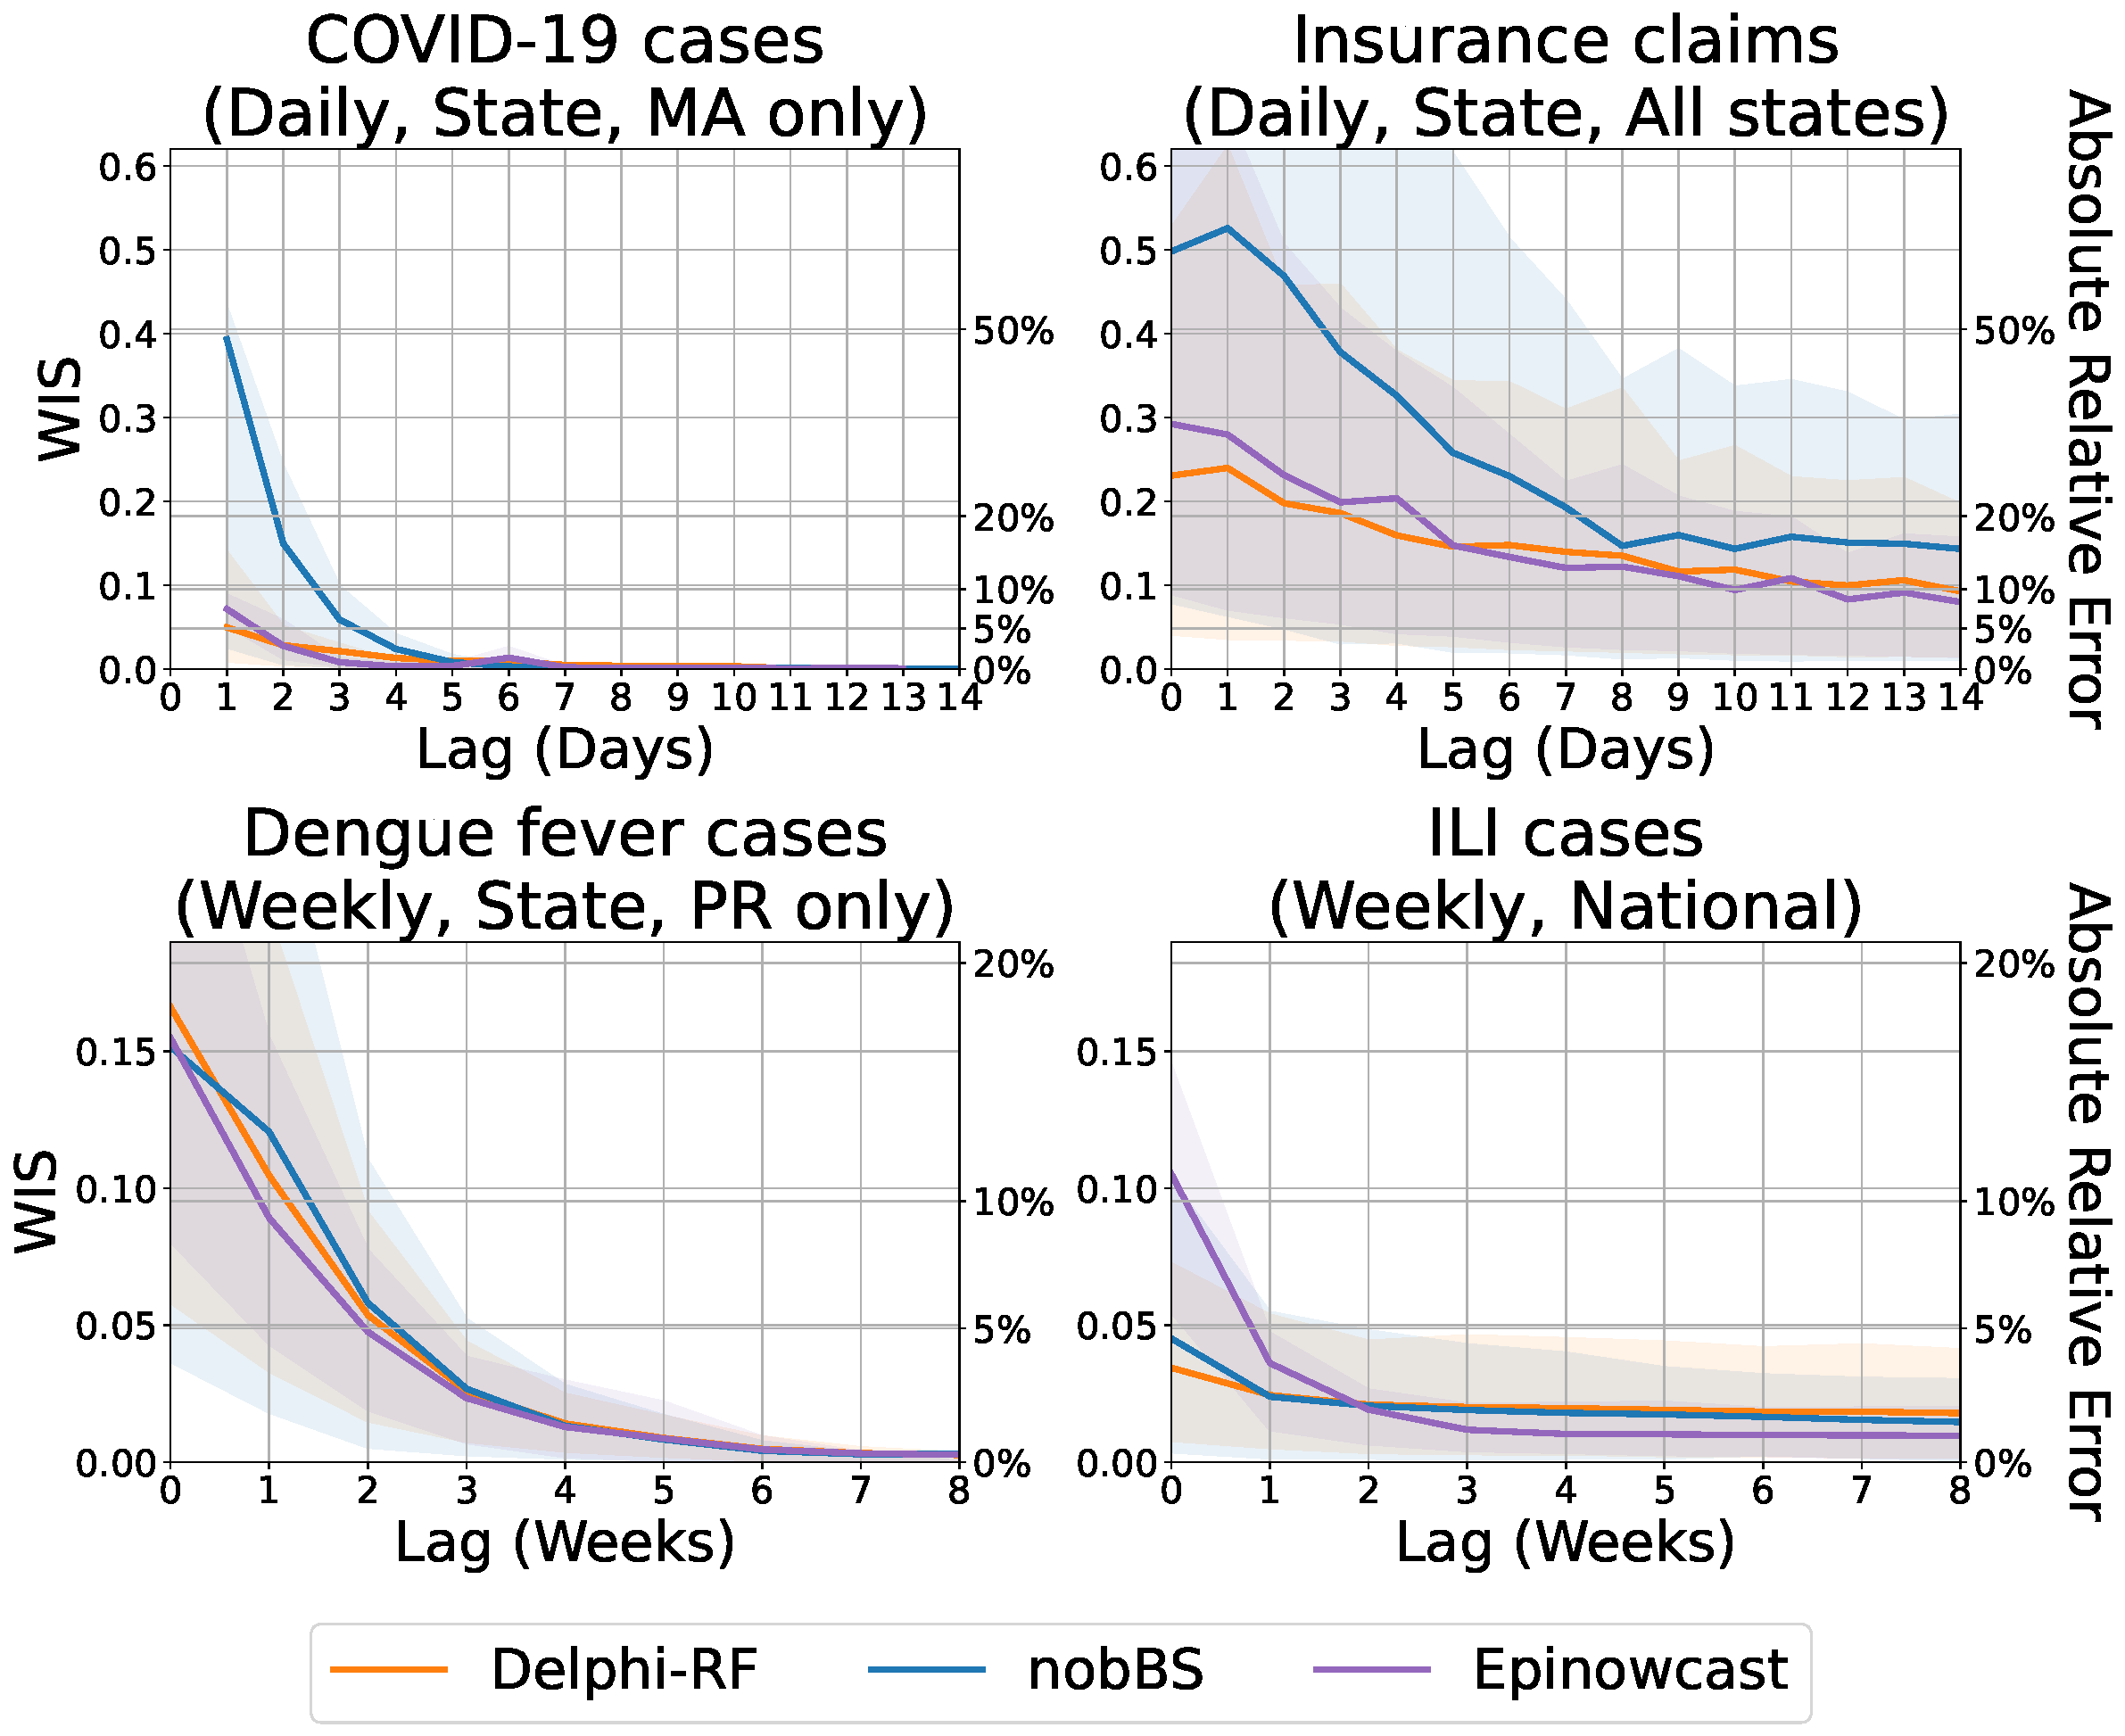
\includegraphics[width=\textwidth]{figs/experiment_count_result_evl_general_for_comparison.pdf}
    \caption{\emph{\textbf{Count forecast evaluation results comparison with nobBS and Epinowcast.} Top: Forecasts of the number of finalized confirmed cases in Massachusetts only and forecasts of the number of insurance claims in all states based on insurance claims data. Bottom: Forecasts of the number of dengue fever cases in Puerto Rico and forecasts of the number of influenza-like illness (ILI) cases nationwide. The solid lines represent the mean WIS, and the absolute relative errors between the most recent report and the target, averaged over locations and reference dates for each lag. The shaded areas represent the 10\% quantile to 90\% quantile.}}
\end{figure}

As shown in Figure 8, our model demonstrated accurate forecasts across all datasets. In general, for daily COVID-19 signals, Delphi-RF consistently outperformed nobBS for daily data and matched or exceeded the accuracy of Epinowcast. For weekly data, Delphi-RF still achieved a comparable level of forecast accuracy, which can be as low as around 10\% absolute relative error when only one revision, one week after the first release, becomes available for dengue fever cases in PR, and even lower than 5\% absolute relative error for national ILI cases.

It is worth noting that our approach leverages the distinct advantages of machine learning models, which can be trained and tested separately, whereas both Epinowcast and nobBS require simultaneous training and forecasting. Our approach has proven to be significantly more efficient. The runtime reported in Table 1 reflects both the training and testing phases required by our model (including the computing time for data pre-processing), which is substantially faster than the other two methods. Furthermore, unlike Epinowcast and nobBS, our approach does not require daily retraining; once trained, the model can be applied repeatedly to produce forecasts for new data without the need for re-estimation. This efficiency enables our model to produce revision forecasts for multiple signals at different temporal resolutions in real time while requiring significantly fewer computational resources.







